\documentclass[14pt]{beamer}
\title{WEB :: CSS}
\author[TS]{TalentSprint}
\institute[L\&D]{Licensed To Skill}
\usefonttheme{serif}
\usecolortheme{orchid}
\usepackage{bookman}
\usepackage{multirow}
\usepackage{fancybox}
\usepackage[percent]{overpic}
\usepackage{hyperref}
\usepackage[T1]{fontenc}
\usepackage{graphicx}
\usepackage{listings}
\graphicspath{{./../Images/}}
\usepackage{tikz}
\usepackage{soul}
\usepackage{color}
\beamertemplateballitem
\usebackgroundtemplate{
\includegraphics[width=\paperwidth]{TS-XP-Logo.jpg}}
\lstset{language=html, numbers=left, numbers=none, basicstyle=\footnotesize, numberstyle=\tiny,  numbersep=10pt, showstringspaces=false, breaklines=true,keepspaces=true, columns=flexible}
\begin{document}

\begin{frame}
  \titlepage
\end{frame}

\begin{frame}{CSS}
The content in this presentation is aimed at teaching  learners to:
  \begin{itemize}
  \item Describe the parts of CSS rules,
  \item Explain how CSS transforms the HTML tags,
  \item Apply different categories of CSS like background, text, font, list
  \end{itemize}
\end{frame}

\begin{frame}{CSS}
Problems of HTML

\vspace{1pc}
\begin{minipage}{1cm}
  \begin{figure}[H]
   \begin{center}
    
\includegraphics[scale=.3]{html-problems.png}
   \end{center}
  \end{figure}
 \end{minipage}
 \quad
 \begin{minipage}{9cm}
 \begin{itemize}
 \item Intended to define content only. Not intended to contain tags for formatting a document. 
 \item Changes to the document is a long and expensive process.
 \item Does not have complete control over the formatting of HTML Document.
\end{itemize}
 \end{minipage}
\end{frame}

\begin{frame}{CSS}
Problems of HTML

\begin{figure}[H]
   \begin{center}
    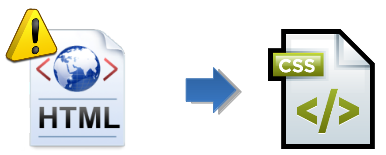
\includegraphics[scale=.35]{problems-of-html.png}
   \end{center}
\end{figure}
\begin{itemize}
 \item To solve this problem, the World Wide Web Consortium (W3C) created CSS.
 \item Purpose of CSS is to store the format part of HTML document.
 \item All browsers support CSS.
\end{itemize}
\end{frame}

\begin{frame}{CSS}
What is CSS?
\begin{itemize}
 \item CSS (Cascading Style Sheets) is a style sheet used for describing the presentation (the look and formatting) of a document.
 \item Enables the separation of document's content from document's presentation, including the elements like, layout, colors, fonts, etc.
\end{itemize}
\end{frame}

\begin{frame}{CSS}
\textbf{Types of CSS}

\vspace{1pc}
There are three types of Style Sheets based on their cascading to HTML Documents:
\begin{enumerate}
 \item Inline Style Sheet
 \item Internal Style Sheet
 \item External Style Sheet
\end{enumerate}
\end{frame}

\begin{frame}{CSS}
\textbf{Inline Style Sheet}

Placing the css code in the (X)html file along side the element for which you want to define a style. 
\begin{block}{Example}
\lstinline!<p style = ``color: \#999999;''>Some gray text</p>!

\color{gray}{Some gray text}
\end{block}

\emph{\textbf{Note:} User cannot change  the styles of elements or text formatted in this way.}
\end{frame}

\begin{frame}[fragile]{CSS}
\textbf{Internal Style Sheet}

Placing the CSS code within the \lstinline!<head></head>! tags of each (X)HTML file.
\begin{block}{Example}
\begin{lstlisting}
<head>
    <title><title>
    <style type = ``text/css''>
        CSS Content Goes Here
    </style>
</head>
\end{lstlisting}
\end{block}
Good if we need to define different style for different pages.
\end{frame}

\begin{frame}{CSS}
\textbf{External Style Sheet}

\begin{itemize}
 \item Website does not contain (X)HTML, instead it uses external CSS document.
 \item Save it with the \lstinline!.css! file extension.
 \item Need to edit only \lstinline!.css! file to make global changes to a website.
\end{itemize}
\end{frame}

\begin{frame}[fragile]{CSS}
\textbf{External Style Sheet}
\begin{block}{Example}
\begin{lstlisting}
<head>
    <title><title>
    <link rel = ``stylesheet'' type = ``text/css'' href = ``style.css''/>
</head>
<body>
\end{lstlisting}
\end{block}
\end{frame}

\begin{frame}{CSS}
Comparing Types of CSS

\begin{figure}[H]
\begin{center}
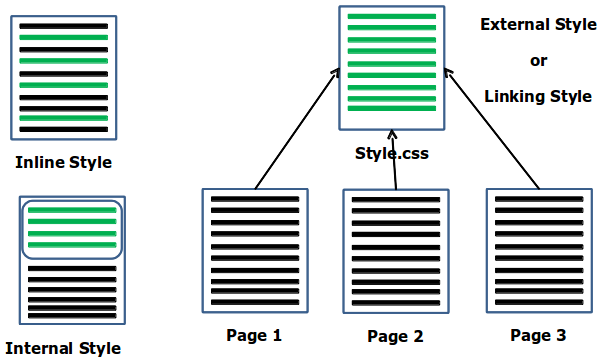
\includegraphics[scale=.4]{compare-styles-css.png}
\end{center}
\end{figure}
\end{frame}

\begin{frame}{CSS}
\textbf{CSS Syntax:} Syntax for CSS is different than that of (X) HTML markup.

\vspace{1pc}
It consists of only 3 parts:
\begin{description}
 \item [Selector] is the (X)HTML element for which you want to apply a style.
 \item [Property] is the actual property title.
 \item [Value] is the style you apply to that property.
\end{description}
\end{frame}

\begin{frame}{CSS}
\textbf{CSS Syntax}

\begin{figure}[H]
\centering
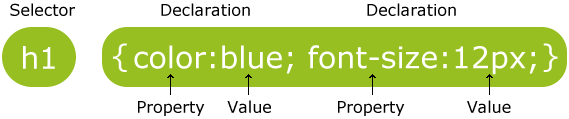
\includegraphics[scale=.4]{css-syntax.png}
\end{figure}
\end{frame}

\begin{frame}{CSS}
CSS Syntax
\begin{itemize}
 \item Each selector can have multiple properties and each property within that selector can have independent values.
 \item The property and value are separated with a colon and contained within curly braces.
 \item Multiple properties are separated by a semi colon.
\end{itemize}
\end{frame}

\begin{frame}[fragile]{CSS}
CSS Syntax
\begin{itemize}
 \item Multiple values within a property are separated by commas.
 \item Individual value containing more than one word should be placed within the double quotes.
 \begin{lstlisting}
  div {
      background: #eeeeee;
      font-family: ``Trebuchet MS'', Verdana, Arial, serif;
  }
 \end{lstlisting}
\end{itemize}
\end{frame}

\begin{frame}[fragile]{CSS}
\textbf{Combining Selectors}

\vspace{1pc}
Combining Elements within one selector:
\begin{lstlisting}
  h1, h2, h3, h4, h5, h6 {
      color: #009900;
      font-family: Georgia, sans-serif;
  }
\end{lstlisting}
All the header elements can be grouped into one selector by using commas to separate each element.
\end{frame}

\begin{frame}{CSS}
\textbf{Comment Tags}
\begin{itemize}
 \item Comment Tags are used to explain why you added certain selectors within your CSS file.

 \item Comments that will be ignored by browsers

 \lstinline!/* This is a comment */!
\end{itemize}
\end{frame}

\begin{frame}{CSS}
\textbf{Backgrounds}

\begin{tabular}{|p{3cm} | p{7cm} |}
\hline
\textbf{Property} & \textbf{Description} \\ \hline
background-attachment &Sets whether a background image is fixed or scrolls with the rest of the page \\ \hline
background-color & Sets the background color of an element \\ \hline
background-image & Sets the background image for an element \\ \hline
background-position & Sets the starting position of a background image \\ \hline
background-repeat & Sets how a background image will be repeated \\ \hline
\end{tabular}
\end{frame}

\begin{frame}{CSS}
\textbf{Text Properties}

\small
\begin{tabular}{|p{3cm} | p{7cm} |}
\hline
\textbf{Property} & \textbf{Description} \\ \hline
color &Sets the color of text \\ \hline
letter-spacing & Increases or decreases the space between characters in a text\\ \hline
line-height & Sets the line height \\ \hline
text-align & Specifies the horizontal alignment of text \\ \hline
text-decoration & Specifies the decoration added to text \\ \hline
text-indent & Specifies the indentation of the first line in a text-block \\ \hline
text-transform & Controls the capitalization of text \\ \hline
word-spacing & Increases or decreases the space between words in a text \\ \hline 
\end{tabular}
\end{frame}

\begin{frame}{CSS}
\textbf{Font Properties}

\vspace{.5pc}

\begin{tabular}{|p{3cm} | p{7cm} |}
\hline
\textbf{Property} & \textbf{Description} \\ \hline
font-size/line-height & Specifies the font size and the line-height. Default value is ``normal''.  \\ \hline
font-family & Specifies the font family. Default value depends on the browser.  \\ \hline
font-style & Specifies the font style. Default value is ``normal''. \\ \hline
font-weight & Specifies the font weight. Default value is ``normal''.  \\ \hline
\end{tabular}
\end{frame}

\begin{frame}{CSS}
\textbf{List Style}

\vspace{1pc}
\begin{tabular}{|p{3cm} | p{7cm} |}
\hline
\textbf{Property} & \textbf{Description} \\ \hline
list-style-type & Specifies the type of list-item marker. \\ \hline
list-style-position & Specifies where to place the list-item marker. \\ \hline
list-style-image & Specifies the type of list-item marker. \\ \hline
\end{tabular}
\end{frame}

\begin{frame}{CSS}
\textbf{Pseudo Elements}

\vspace{.5pc}
\fbox{selector : pseudo-element {property: value}}
 
 \vspace{1pc}
\begin{tabular}{|p{3cm} | p{7cm} |}
\hline
\textbf{Property} & \textbf{Description} \\ \hline
first-line & Adds style to the first line of text in a block level element. \\ \hline
first-letter & Adds style to the first letter of text in a block level element. \\ \hline
\end{tabular}
\end{frame}

\begin{frame}{CSS}
\textbf{Pseudo Elements}

\vspace{2pc}
\fbox{p:first-line {font-size: medium; color: \#ff0000;}}

\vspace{2pc}
\fbox{p:first-letter {font-size: medium; color: \#ff0000;}}
\end{frame}

\begin{frame}{CSS}
 \begin{figure}[H]
 \begin{center}
   
\includegraphics[scale=.3]{qa.png}   
 \end{center}
  \end{figure}
\end{frame}

\end{document}
